\documentclass[a4paper,10pt]{article}
\usepackage[spanish,activeacute,es-tabla]{babel}
\usepackage[utf8]{inputenc}
\usepackage{ifthen}
\usepackage{listings}
\usepackage{dsfont}
\usepackage{subcaption}
\usepackage{amsmath}
\usepackage[top=1cm,bottom=2cm,left=1cm,right=1cm]{geometry}%
\usepackage{color}%
\usepackage{changepage}
\newcommand{\tocarEspacios}{%
	\addtolength{\leftskip}{3em}%
	\setlength{\parindent}{0em}%
}

% Especificacion de procs

\newcommand{\In}{\textsf{in }}
\newcommand{\Out}{\textsf{out }}
\newcommand{\Inout}{\textsf{inout }}

\newcommand{\encabezadoDeProc}[4]{%
	% Ponemos la palabrita problema en tt
	%  \noindent%
	{\normalfont\bfseries\ttfamily proc}%
	% Ponemos el nombre del problema
	\ %
	{\normalfont\ttfamily #2}%
	\
	% Ponemos los parametros
	(#3)%
	\ifthenelse{\equal{#4}{}}{}{%
		% Por ultimo, va el tipo del resultado
		\ : #4}
}

\newenvironment{proc}[4][res]{%
	
	% El parametro 1 (opcional) es el nombre del resultado
	% El parametro 2 es el nombre del problema
	% El parametro 3 son los parametros
	% El parametro 4 es el tipo del resultado
	% Preambulo del ambiente problema
	% Tenemos que definir los comandos requiere, asegura, modifica y aux
	\newcommand{\requiere}[2][]{%
		{\normalfont\bfseries\ttfamily requiere}%
		\ifthenelse{\equal{##1}{}}{}{\ {\normalfont\ttfamily ##1} :}\ %
		\{\ensuremath{##2}\}%
		{\normalfont\bfseries\,\par}%
	}
	\newcommand{\asegura}[2][]{%
		{\normalfont\bfseries\ttfamily asegura}%
		\ifthenelse{\equal{##1}{}}{}{\ {\normalfont\ttfamily ##1} :}\
		\{\ensuremath{##2}\}%
		{\normalfont\bfseries\,\par}%
	}
	\renewcommand{\aux}[4]{%
		{\normalfont\bfseries\ttfamily aux\ }%
		{\normalfont\ttfamily ##1}%
		\ifthenelse{\equal{##2}{}}{}{\ (##2)}\ : ##3\, = \ensuremath{##4}%
		{\normalfont\bfseries\,;\par}%
	}
	\renewcommand{\pred}[3]{%
		{\normalfont\bfseries\ttfamily pred }%
		{\normalfont\ttfamily ##1}%
		\ifthenelse{\equal{##2}{}}{}{\ (##2) }%
		\{%
		\begin{adjustwidth}{+5em}{}
			\ensuremath{##3}
		\end{adjustwidth}
		\}%
		{\normalfont\bfseries\,\par}%
	}
	
	\newcommand{\res}{#1}
	\vspace{1ex}
	\noindent
	\encabezadoDeProc{#1}{#2}{#3}{#4}
	% Abrimos la llave
	\par%
	\tocarEspacios
}
{
	% Cerramos la llave
	\vspace{1ex}
}

\newcommand{\aux}[4]{%
	{\normalfont\bfseries\ttfamily\noindent aux\ }%
	{\normalfont\ttfamily #1}%
	\ifthenelse{\equal{#2}{}}{}{\ (#2)}\ : #3\, = \ensuremath{#4}%
	{\normalfont\bfseries\,;\par}%
}

\newcommand{\pred}[3]{%
	{\normalfont\bfseries\ttfamily\noindent pred }%
	{\normalfont\ttfamily #1}%
	\ifthenelse{\equal{#2}{}}{}{\ (#2) }%
	\{%
	\begin{adjustwidth}{+2em}{}
		\ensuremath{#3}
	\end{adjustwidth}
	\}%
	{\normalfont\bfseries\,\par}%
}

% Tipos

\newcommand{\nat}{\ensuremath{\mathds{N}}}
\newcommand{\ent}{\ensuremath{\mathds{Z}}}
\newcommand{\float}{\ensuremath{\mathds{R}}}
\newcommand{\bool}{\ensuremath{\mathsf{Bool}}}
\newcommand{\cha}{\ensuremath{\mathsf{Char}}}
\newcommand{\str}{\ensuremath{\mathsf{String}}}

% Logica

\newcommand{\True}{\ensuremath{\mathrm{true}}}
\newcommand{\False}{\ensuremath{\mathrm{false}}}
\newcommand{\Then}{\ensuremath{\rightarrow}}
\newcommand{\Iff}{\ensuremath{\leftrightarrow}}
\newcommand{\implica}{\ensuremath{\longrightarrow}}
\newcommand{\IfThenElse}[3]{\ensuremath{\mathsf{if}\ #1\ \mathsf{then}\ #2\ \mathsf{else}\ #3\ \mathsf{fi}}}
\newcommand{\yLuego}{\land _L}
\newcommand{\oLuego}{\lor _L}
\newcommand{\implicaLuego}{\implica _L}

\newcommand{\cuantificador}[5]{%
	\ensuremath{(#2 #3: #4)\ (%
		\ifthenelse{\equal{#1}{unalinea}}{
			#5
		}{
			$ % exiting math mode
			\begin{adjustwidth}{+2em}{}
				$#5$%
			\end{adjustwidth}%
			$ % entering math mode
		}
		)}
}

\newcommand{\existe}[4][]{%
	\cuantificador{#1}{\exists}{#2}{#3}{#4}
}
\newcommand{\paraTodo}[4][]{%
	\cuantificador{#1}{\forall}{#2}{#3}{#4}
}

%listas

\newcommand{\TLista}[1]{\ensuremath{seq \langle #1\rangle}}
\newcommand{\lvacia}{\ensuremath{[\ ]}}
\newcommand{\lv}{\ensuremath{[\ ]}}
\newcommand{\longitud}[1]{\ensuremath{|#1|}}
\newcommand{\cons}[1]{\ensuremath{\mathsf{addFirst}}(#1)}
\newcommand{\indice}[1]{\ensuremath{\mathsf{indice}}(#1)}
\newcommand{\conc}[1]{\ensuremath{\mathsf{concat}}(#1)}
\newcommand{\cab}[1]{\ensuremath{\mathsf{head}}(#1)}
\newcommand{\cola}[1]{\ensuremath{\mathsf{tail}}(#1)}
\newcommand{\sub}[1]{\ensuremath{\mathsf{subseq}}(#1)}
\newcommand{\en}[1]{\ensuremath{\mathsf{en}}(#1)}
\newcommand{\cuenta}[2]{\mathsf{cuenta}\ensuremath{(#1, #2)}}
\newcommand{\suma}[1]{\mathsf{suma}(#1)}
\newcommand{\twodots}{\ensuremath{\mathrm{..}}}
\newcommand{\masmas}{\ensuremath{++}}
\newcommand{\matriz}[1]{\TLista{\TLista{#1}}}
\newcommand{\seqchar}{\TLista{\cha}}

\renewcommand{\lstlistingname}{Código}
\lstset{% general command to set parameter(s)
	language=Java,
	morekeywords={endif, endwhile, skip},
	basewidth={0.47em,0.40em},
	columns=fixed, fontadjust, resetmargins, xrightmargin=5pt, xleftmargin=15pt,
	flexiblecolumns=false, tabsize=4, breaklines, breakatwhitespace=false, extendedchars=true,
	numbers=left, numberstyle=\tiny, stepnumber=1, numbersep=9pt,
	frame=l, framesep=3pt,
	captionpos=b,
}
\usepackage{changepage}
\usepackage{xcolor}
\usepackage[T1]{fontenc}
\usepackage{listings}
\usepackage{color}
\usepackage{amssymb}

\definecolor{dkgreen}{rgb}{0,0.6,0}
\definecolor{gray}{rgb}{0.5,0.5,0.5}
\definecolor{mauve}{rgb}{0.58,0,0.82}

\lstset{frame=tb,
  language=Java,
  aboveskip=3mm,
  belowskip=3mm,
  showstringspaces=false,
  columns=flexible,
  basicstyle={\small\ttfamily},
  numbers=none,
  numberstyle=\tiny\color{gray},
  keywordstyle=\color{blue},
  commentstyle=\color{dkgreen},
  stringstyle=\color{mauve},
  breaklines=true,
  breakatwhitespace=true,
  tabsize=3
}
\newcommand{\noexiste}[4][]{%
	\cuantificador{#1}{\nexists}{#2}{#3}{#4}
}
\renewcommand*\ttdefault{txtt}
\renewcommand*\familydefault{\ttdefault} %% Only if the base font of the document is to be typewriter style
\newcommand{\tbft}[2]{\par\addvspace{\baselineskip}\textbf{#1}\hspace{0.35em}{#2}\\\par\addvspace{\baselineskip}}
\newcommand{\ejercicio}[2]{\par\addvspace{\baselineskip}\textbf{Ejercicio #1.}\hspace{0.35em}{#2}\\\par\addvspace{\baselineskip}}
% \ejercicio{NUMERO}{ENUNCIADO}
%   Devuelve
% Ejercicio NUMERO. ---- ENUNCIADO ----
%
%formato
\newcommand{\salto}[1]{\par\addvspace{#1}}
\newcommand{\rojo}[1]{{\color{red}#1}}
\newcommand{\anotacion}[2][red]{\salto{1ex}\noindent\texttt{\color{#1}#2}\salto{1ex}}
\newcommand{\anotacionns}[2][red]{\noindent\texttt{\color{#1}#2}}
\newcommand{\return}{\textbf{return }}
%
% si y solo si corto y largo
\newcommand{\sii}{\leftrightarrow}
\newcommand{\siiLargo}{\longleftrightarrow}
\newcommand{\slr}[1]{\ensuremath{\langle #1\rangle}}
\newcommand{\smm}[1]{\textless #1\textgreater}
\newcommand{\encabezadoTAD}[1]{\par\salto{1ex}\noindent TAD\ \ \normalfont\ttfamily#1 }
\newenvironment{tad}[1]{
\newcommand{\nombretad}{{\ttfamily#1}}
\newcommand{\nt}{\nombretad}
\newcommand{\obs}[2]{\par\noindent{\ttfamily obs} ##1: ##2\par}
\encabezadoTAD{#1}\{
    \begin{adjustwidth}{3em}{0em}}
{\end{adjustwidth}\par\}}
% \begin{tad}{nombre del tad}
%   AGREGAR UN OBSERVADOR
%     \obs{nombre observador}{tipo}
%     \nombretad <---------- DEVUELVE EL NOMBRE DEL TAD (du)
%
%   y aca se pueden usar todos los procs y cosas de la catedra
%
%     \end{tad}
\newcommand{\encabezadoImpl}[3]{\par\salto{1ex}\noindent \textbf{impl}\ \normalfont\ttfamily#1(#2):#3}
\newcommand{\asg}[2]{\salto{0em}\noindent{\ttfamily #1}:= #2\salto{0em}}
\newcommand{\asgns}[2]{\noindent{\ttfamily #1}:= #2}
\newenvironment{impl}[3]{\encabezadoImpl{#1}{#2}{#3}\{
\begin{adjustwidth}{3em}{0em}
}
{\end{adjustwidth}\par\}}
\newcommand{\encabezadoDesign}[2]{\par\salto{1ex}\noindent \textbf{modulo}\ {\normalfont\ttfamily #1} \textbf{implementa}{ \normalfont\ttfamily #2}}
\newenvironment{design}[2]{\encabezadoDesign{#1}{#2}\{
\newcommand{\var}[2]{\salto{0em}\noindent{\normalfont \bfseries var} \texttt{##1}: \texttt{##2}\salto{0em}}
\begin{adjustwidth}{3em}{0em}
}
{\end{adjustwidth}\}}
\newcommand{\ifthel}[3]{\salto{0ex}
\noindent{\normalfont \bfseries if}{ #1 }{\normalfont \bfseries then}\salto{0ex}
\noindent{\begin{adjustwidth}{1.5em}{0em}#2\end{adjustwidth}}\salto{0ex}
\noindent{\normalfont \bfseries else}\begin{adjustwidth}{1.5em}{0em}{#3}\end{adjustwidth}\salto{0ex}
\noindent{\bfseries end if}}\salto{0ex}
\newcommand{\while}[2]{
    \salto{0em}\noindent
    {\normalfont \bfseries while} \ensuremath{#1} \textbf{do}
    \begin{adjustwidth}{1.5em}{0em}{#2}\end{adjustwidth}\salto{0em}\noindent{\normalfont \bfseries end while}
}
\newcommand{\invrep}[2]{\salto{0em}\noindent{\bfseries pred} InvRep (#1)\{\salto{0em}\noindent\begin{adjustwidth}{2em}{0em}{#2}\end{adjustwidth}\salto{0em}\noindent\}}
\newcommand{\abs}[2]{\salto{0em}\noindent{\bfseries pred} Abs (#1)\{\salto{0em}\noindent\begin{adjustwidth}{2em}{0em}{#2}\end{adjustwidth}\salto{0em}\noindent\}}

\usepackage[dvipsnames]{xcolor}
\usepackage{graphicx}
\usepackage{microtype}
\geometry{
    a4paper,
    total={170mm,257mm},
    left=5mm,
    top=10mm,
    }
\graphicspath{{images/}}
\begin{document}
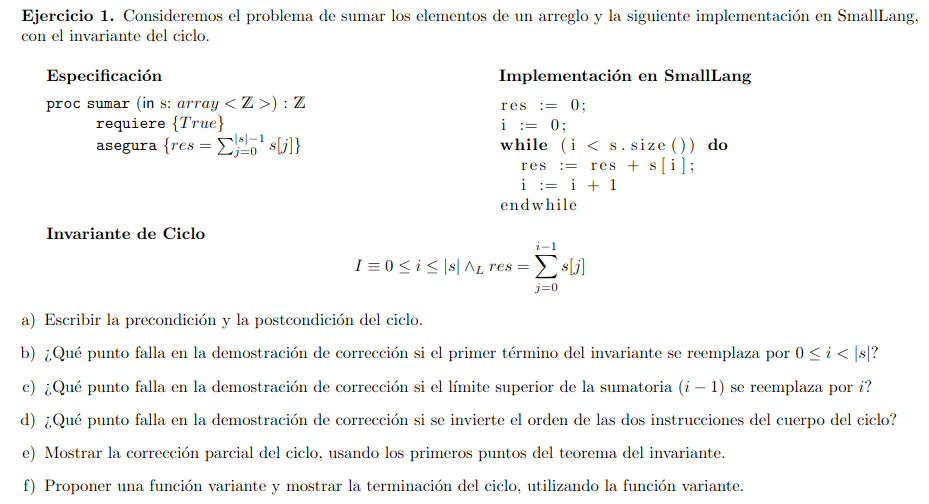
\includegraphics[width=\textwidth]{e1.png}
a) La poscondicion del ciclo sera la misma que el \emph{asegura} de la especificacion, $res=\sum_{j=0}^{i-1}s[j]$

La precondicion por otro lado no estoy seguro, sera que res=0 y i=0(las primeras dos lineas de S)?

Could be

b) de reemplazarse el primer termino del invariante este fallaria a la hora de mantenerse cierto al salir del ciclo

Esto pues el while aumenta i en uno |s| veces, donde la |s|-ava vez no entra al ciclo y el programa termina.

c) Deja de ser cierto durante toda la ejecucion del programa, basicamente te esta pidiendo que el termino que el programa esta por sumar ya este sumado a res

d) Al llegar a la ultima iteracion se intentaria acceder a un elemento del arreglo que no existe?¿? creo

f) \begin{itemize}
    \item $Pc\implies I$

          $res=0 \land i=0 \implies 0\leq i \leq |s| \land_L res=\sum_{j=0}^{i-1}s[j]$

          $res=0 \land i=0 \implies 0\leq 0 \leq |s| \land_L 0=\sum_{j=0}^{1-1}$

          $res=0 \land i=0 \implies true$

    \item $\{I\land B\}S\{I\}$

          {\color{blue}\{$0\leq i \leq |s| \land_L res=\sum_{j=0}^{i-1}s[j] \land i<|s|\}\equiv \{0\leq i < |s| \land_L res=\sum_{j=0}^{i-1}s[j]\}$}

          res:= res + s[i]

          i:=i+1

          ${\color{blue}\{0\leq i \leq |s| \land_L res=\sum_{j=0}^{i-1}s[j]\}}$

          Esto se traduce a comparar la primera parte de la tripla de Hoare con wp(res:=res+s[i]; i:=i+1, I)

          ${\color{blue}\{0\leq i<|s| \land_L 0\leq i+1 \leq |s| \land_L res+s[i]=\sum_{j=0}^{i}s[j]\}}$

          ${\color{blue}\equiv\{ 0\leq i<|s| \land_L -1\leq i \leq |s|-1 \land_L res=\sum_{j=0}^{i-1}s[j]\}}$

          ${\color{blue}\equiv\{ 0\leq i < |s| \land_L res=\sum_{j=0}^{i-1}s[j]\}}$

          Y podemos ver que ambos $I\land B$ y la wp calculada son iguales, por lo tanto la tripla de Hoare es correcta

    \item $I \land \lnot B \implies Q_c$

          $0\leq i \leq |s| \land_L res=\sum_{j=0}^{i-1}s[j] \land \lnot (i<|s|)$

          $\equiv 0\leq i \leq |s| \land_L res=\sum_{j=0}^{i-1}s[j] \land i\geq|s|$

          $\equiv i = |s| \land_L res=\sum_{j=0}^{i-1}s[j]$

          $\equiv res=\sum_{j=0}^{|s|-1}s[j]$

          Que es efectivamente nuestra postcondicion de la especificacion.
\end{itemize}
\pagebreak

f)  Propuesta 1: $fv=|s|-i+1$

\salto{\baselineskip}

$\{I\land B \land v_0=fv\} res:=res+s[i];i:=i+1 \{fv<v_0\}\equiv Pc\implies wp(s,fv<v_0)$

\salto{\baselineskip}

$wp(S,fv<v_0)\equiv wp(res:=res+s[i], wp(i:=i+1, |s|-i+1<v_0))$

cosas...

\hspace*{2em}$\equiv |s|-(i+1)+1<v_0 \equiv |s|-i<v_0$

\salto{\baselineskip}

retomando el principio:

$I\land B \land v_0=fv \implies |s|-i<v_0$?

Si, pues $ v_o=fv \implies |s|-i<|s|-i+1$ que es trivialmente cierto.

Ahora, mi propuesta cumple con el segundo statement?

$I \land fv\leq 0 \implies \lnot B$

$\alpha:\ |s|-i+1\leq 0 \implies |s|+1\leq i$

$\beta:\ \lnot B \equiv i\geq |s| \equiv |s|\leq i\hspace*{5em} \longleftarrow $A lo que quiero llegar

$I\equiv 0\leq i \leq |s| \land_L res=\sum_{j=0}^{i-1}s[j]$

Tengo informacion de sobra, $\alpha \implies |s| \leq i \equiv \lnot B$

Seems a bit too easy pero es el primer ejercicio de la guia so...


\pagebreak


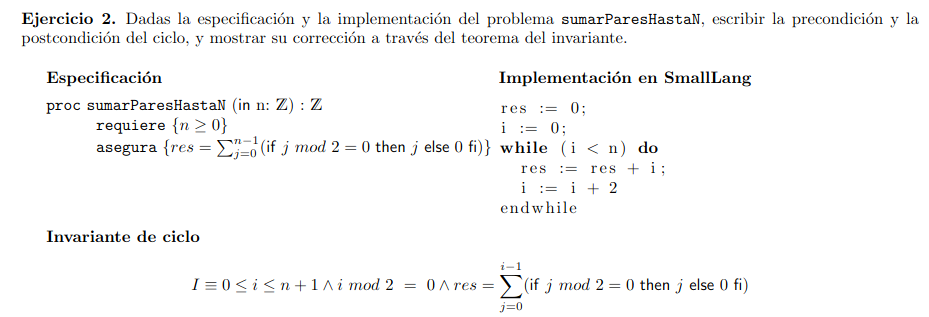
\includegraphics[width=\textwidth]{e2.png}

La precondicion del ciclo seria ...........................

La poscondicion es $res=\sum_{j=0}^{n-1}if\ j\ mod 2 = 0\ then\ j\ else\ 0$

$P\implies I$ es trivialmente cierto

\salto{\baselineskip}

$2^{da})$$\{I \land B \} res:=res+i; i:=i+2\{I\}$

    \salto{\baselineskip}

$I\equiv 0\leq i\leq n+1 \land i\%2=0 \land res=\sum_{j=0}^{i-1}if\ j\%2 = 0\ then\ j\ else\ 0$ {\small {\color{Violet}$\hfill \leftarrow$Por las dudas: Uso $\%$ en lugar de mod por cuestiones de spacing}}

$B\equiv i<n$

$wp(S,I)\equiv 0\leq i\leq n+1 \land i\%2=0 \land res+i=\sum_{j=0}^{i+1}if\ j\%2 = 0\ then\ j\ else\ 0$

Analizando un poco nos damos cuenta de que i siempre sera par, por lo que i+1 es impar, entonces el termino i+1 de la sumatoria siempre sumara 0 (por el condicional), asi que podemos obviarlo. A su vez, podemos restar a ambos lados el termino i-esimo, que este sera par y por lo tanto si contara en la sumatoria, simplificando la expresion.

$wp(S,I)\equiv 0\leq i\leq n+1 \land i\%2=0 \land res=\sum_{j=0}^{i-1}if\ j\%2 = 0\ then\ j\ else\ 0$

Entonces, $I\land B \equiv 0\leq i<n \land i\%2=0 \land res=\sum_{j=0}^{i-1}if\ j\%2 = 0\ then\ j\ else\ 0$

Que efectivamente implica mi wp, pues el segundo termino es identico y en el primero,

$0\leq i<n\implies 0\leq i\leq n+1$

\salto{\baselineskip}

$3^{ra})\ I\land\lnot B\implies Q_c$

$I\equiv 0\leq i\leq n+1 \land i\%2=0 \land res=\sum_{j=0}^{i-1}if\ j\%2 = 0\ then\ j\ else\ 0$

$\lnot B\equiv i\geq n$

$n\leq i \land i\leq n+1\equiv n\leq i\leq n+1$

Pero i tiene que ser par, por lo que: $n\leq i\leq n+1\equiv n=i=n \equiv i=n$

$i=n \land i\%2=0 \land res=\sum_{j=0}^{i-1}if\ j\%2 = 0\ then\ j\ else\ 0 \equiv res=\sum_{j=0}^{n-1}if\ j\%2 = 0\ then\ j\ else\ 0 \equiv Q_c$

Posible invariante: $n-i+1$

$\{I\land B\land v_0=fv\} S \{fv<v_0\}$

$wp(i:=i+2, n-i+1<v_0)\equiv n-i-1<v_0$

entonces $v_0=fv \implies n-i-1<n-i+1$

$5^{ta})\ I\land fv\leq 0 \implies \lnot B$

Quiero entonces llegar a $\lnot B \equiv i\geq n$

$fv\leq 0 \implies n+1\leq i$

$I\implies 0\leq i\leq n+1$

Estas dos cosas implican que $i=n+1$ que a su vez implica $i\geq n$

De forma un poco confusa y poco organizada, pero queda entonces demostrada la correctitud del ciclo.
\pagebreak
\end{document}